\documentclass[../ds]{subfiles}
\begin{document}
\chapter{Fourier Transform}
\begin{itemize}
\item 
Let $x(t)$ be a complex-valued function. Then its Fourier transform is 
\[ X(\omega) = \int_{-\infty}^\infty x(t)e^{-i\omega t}\,dt. \]
The inverse Fourier transform is
\[ x(t) = \frac{1}{2\pi} \int_{-\infty}^\infty X(\omega)e^{i\omega t}\,d\omega. \]

\item 
For a sequence of discrete time signals, use discrete-time Fourier transform:
\[ X(\omega) = \sum_{-\infty}^\infty x[n]e^{-i\omega n}. \]
The output is continuous in $\omega$ and periodic. The inverse DTFT is:
\[ x[n] = \frac{1}{2\pi} \int_{2\pi} X(\omega)e^{i\omega n}\,d\omega. \]

\item
Discrete Fourier transform converts a finite sequence of equally-spaced samples of a function into a same-length sequence of equally-spaced samples of the DTFT. It is given by
\begin{align*} X[k] &= \sum_{n=0}^{N-1} x[n]e^{-2\pi i kn/N} \\&= \sum_{n=0}^{N-1} x[n]W_N^{kn},
\end{align*}
where $W_N = e^{-2\pi i/N}.$
The inverse transform is given by 
\[ \frac{1}{N} \sum_{k=0}^{N-1} X[k]W^{-kn}_N.\]

\item 
The fast Fourier transform is based on the idea that the $N$-th roots of unity $W_N^k$ have nice properties when $N$ is a power of $2.$ In vector form,
\[ \mathbf{X}[k] = \mathbf{W_N}\mathbf{x}[n], \]
where $W_N = V(W_N^0,\ldots,W_N^{N-1})$ is a Vandermonde matrix. The computational complexity is $O(N\log{N})$ vs.\ $O(N^2)$ of definition of DFT.

\item 
Limitation of Fourier transform is that it lacks temporal resolution. A way to overcome this is the short-time Fourier transform.
	\begin{itemize}
	\item 
	Continuous case:
	\[ \STFT\{x(t)\}(\tau, \omega) = \int_{-\infty}^{\infty} x(t)w(t - \tau)e^{-i\omega t}\,dt, \] where $w$ is the window function, usually Hann or Gaussian window.
	
	\item 
	Discrete case:
	\[ \STFT\{x[n]\}(k, \omega) = \sum_{n=-\infty}^{\infty} x[n]w[n-k]e^{-i\omega n}. \]
	\end{itemize}
Uncertainty principle: there is a trade-off between temporal and frequency resolution.

\begin{figure}[ht]
	\centering
	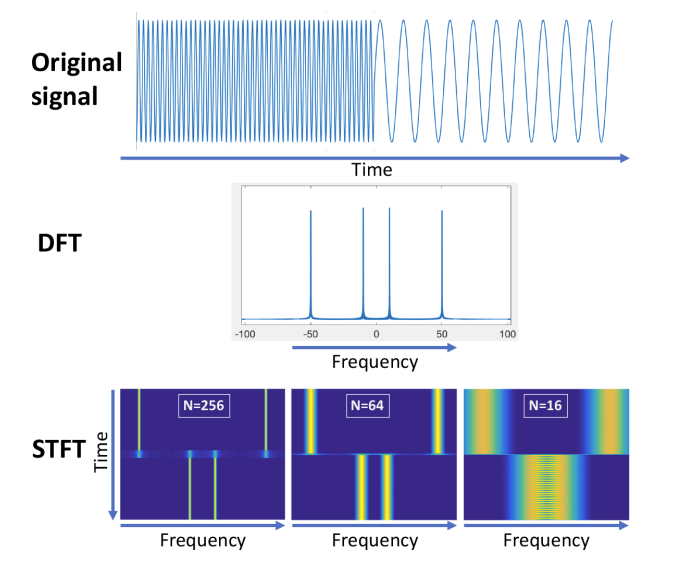
\includegraphics[width=10cm]{fourier_uncertainty}
	\caption*{Image source: \cite{fourier_qiml}}
\end{figure}

\item 
Spectrograms:
	\begin{itemize}
	\item 
	Divide a time-domain signal into segments of equal length.
	
	\item 
	Apply FFT to each segment, transforming the data from the time domain to the frequency domain.
	
	\item 
	Each segment corresponds to vertical line in spectogram.
	
	\item 
	For window width $w,$ $\text{spectogram}(t) = |\STFT(t)|^2.$
	\end{itemize}

\item 
Nyquist–Shannon sampling theorem
	\begin{itemize}
	\item 
	Sampling rate must be at least twice the bandwidth of the signal to avoid aliasing.
	
	\item 
	Let $x(t)$ have Fourier transform $X(f).$ Suppose $X_{1/T}(f)$ is the DTFT of sample sequence $x[n].$ 
	
	\item 
	For DTFT, copies of $X_f$ are shifted by multiples of the sampling rate $f_s$ and added.
	
	\item
	If Nyquist–Shannon is not satisfied, copies will overlap.
	
	\item 
	Any frequency component above $f_s/2$ is indistinguishable from a lower-frequency component (i.e., alias).
	\end{itemize}
\end{itemize}
\end{document}